\documentclass[aspectratio=169]{beamer}
\usepackage{ITMOtheme}
\usepackage{xspace}
\usepackage{array}
\usepackage{pgfplots}
\usepgfplotslibrary{statistics}
\usetikzlibrary{calc,patterns,intersections,shapes.geometric}
\usetikzlibrary{arrows.meta}
\tikzset{%
  >={Latex[width=2mm,length=2mm]},
    base/.style = {
        rectangle, rounded corners, draw=black,
        minimum width=2.7cm, minimum height=1cm,
        text centered, font=\sffamily
    },
    start/.style = {base, fill=blue!30},
    iterate/.style = {base, fill=green!30},
    done/.style = {base, fill=red!30}
}

\newcommand{\hamming}{\textsc{Hamming}\xspace}
\newcommand{\onemax}{\textsc{OneMax}\xspace}
\newcommand{\jump}{\textsc{Jump}\xspace}
\newcommand{\realjump}{\textsc{RealJump}\xspace}
\newcommand{\ollga}{$(1 + (\lambda, \lambda))$~GA\xspace}
\newcommand{\mpoga}{$(\mu + 1)$~GA\xspace}
\newcommand{\todo}[1]{\textbf{\textcolor{red}{TODO: #1}}}

\setfootlinetext{\insertsection \ifx\insertsubsection\empty \else \ / \insertsubsection \fi}

\begin{document}

\begin{frame}[plain]
	\itmopolygons{
	    \begin{center}
	        \vfill
    		\usebeamerfont{titlegraphic}{
\includegraphics[scale=.8]{itmo/logo_en_vert_blue.pdf}}
    		\vfill
    		\usebeamerfont{title}{Lab 1 \& 2} 
    		\vfill
    		\usebeamerfont{subtitle}{Sentiment Analysis of Microblog Data Streams} 
    		\vfill
            Simon Naumov, M4138
		\end{center}
	}
\end{frame}

\begin{frame}
    \frametitle{Using prepared helpful data}
    
    \begin{columns}[c] 
        \column{.5\textwidth}{
            \begin{itemize}[<+->]
                \item \emph{Natural Language Toolkit} library with words, punctuation and stop words
                \item \emph{Regular expressions} for urls, emojis, hashtags, emails and many more metadata
                \item \emph{Contraction} and \emph{emoticons} mappings
            \end{itemize}
        }
        
        \column{.5\textwidth}{
            \begin{overprint}
                \only<1>{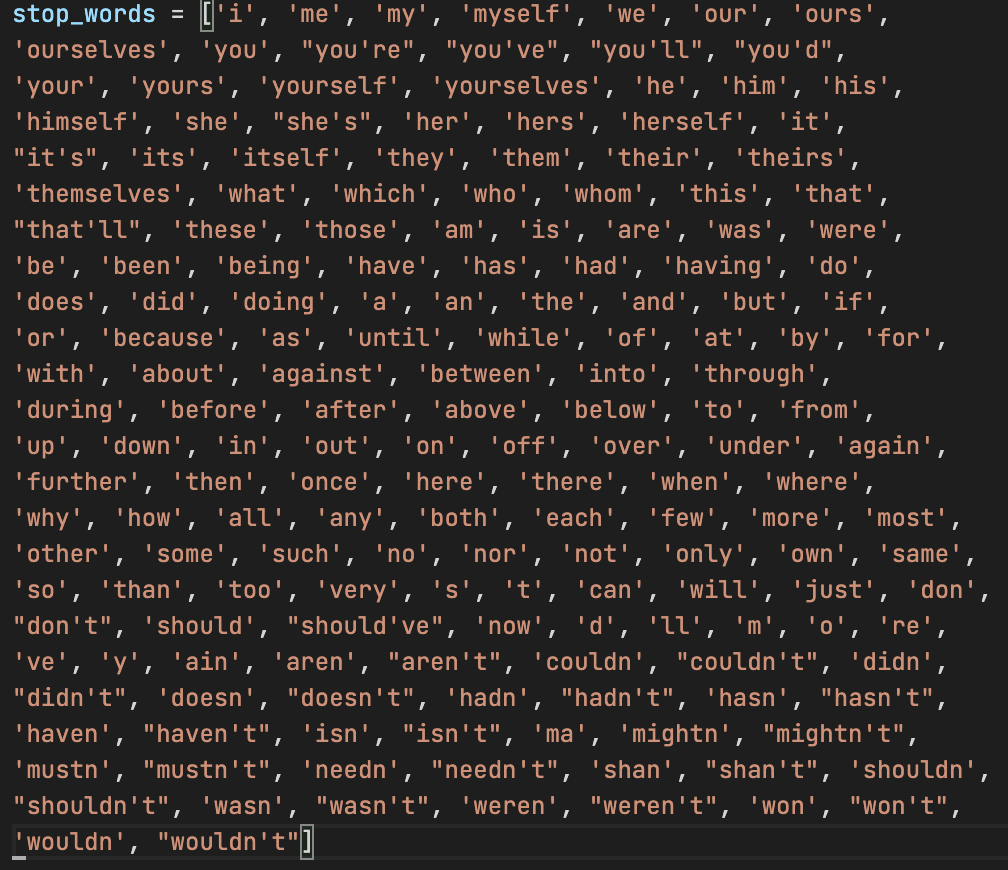
\includegraphics[height=0.75\textheight]{pic/stop_words.png}}
                \only<2>{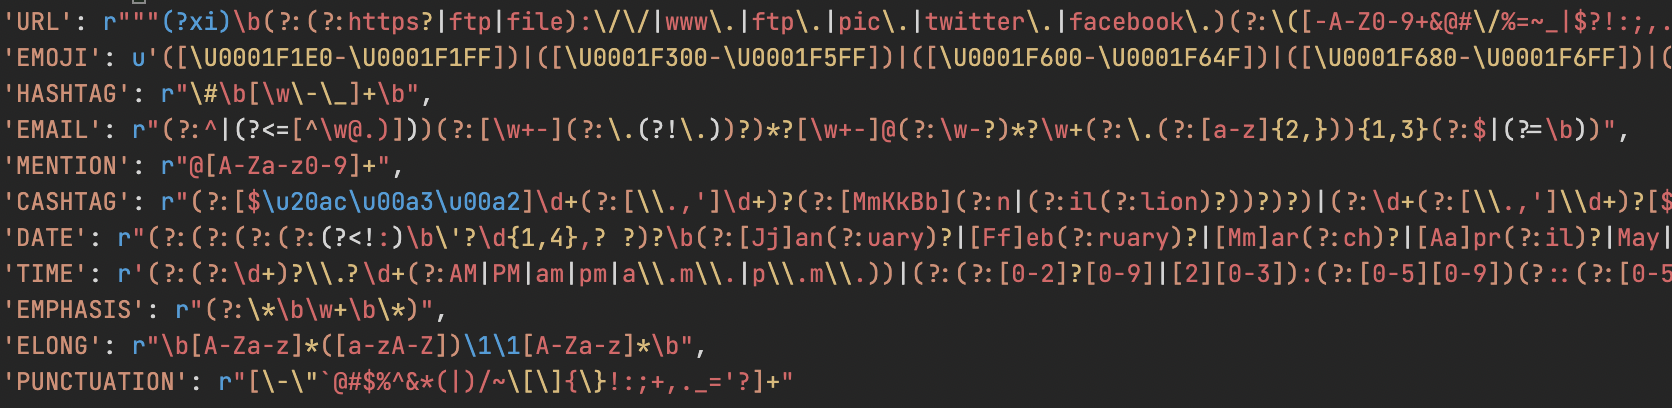
\includegraphics[width=1\textwidth]{pic/regexps.png}}
                \only<3>{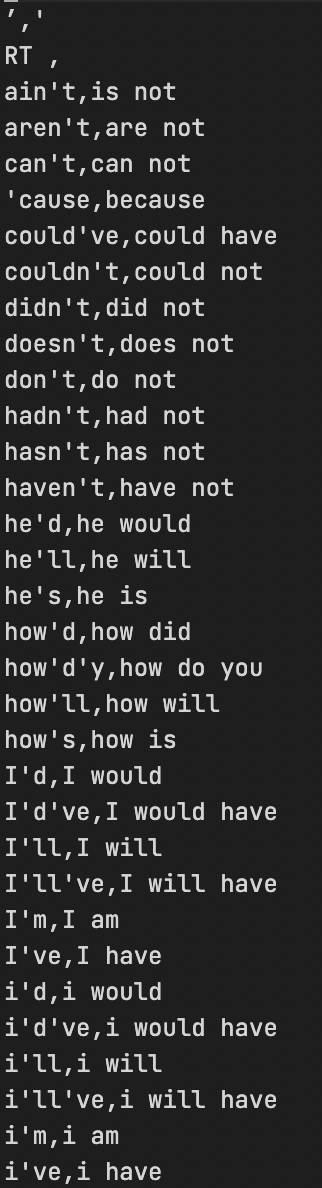
\includegraphics[height=0.85\textheight]{pic/contractions.png}}
                \only<4>{
                    \makebox(10,10){\put(0,-6.2\normalbaselineskip){
                        $\left.\rule{0pt}{3.8\normalbaselineskip}\right\}$
                        normalized string
                    }}
                }
            \end{overprint}
        }
    \end{columns}
\end{frame}

\begin{frame}
    \frametitle{Application}
    
    Machine learning algorithm application with the transformed data input
    
    In particular, train and test \emph{Linear Support Vector Classification}
\end{frame}

\begin{frame}
    \frametitle{Results}
  
    \vspace{2ex}
    
    \begin{columns}[c] 
        \column{.4\textwidth}{
            \begin{itemize}[<+->]
                \item Organization Prediction
                \item Sentiment Analysis
            \end{itemize}
        }
        
        \column{.6\textwidth}{
          \begin{overprint}
            \only<1>{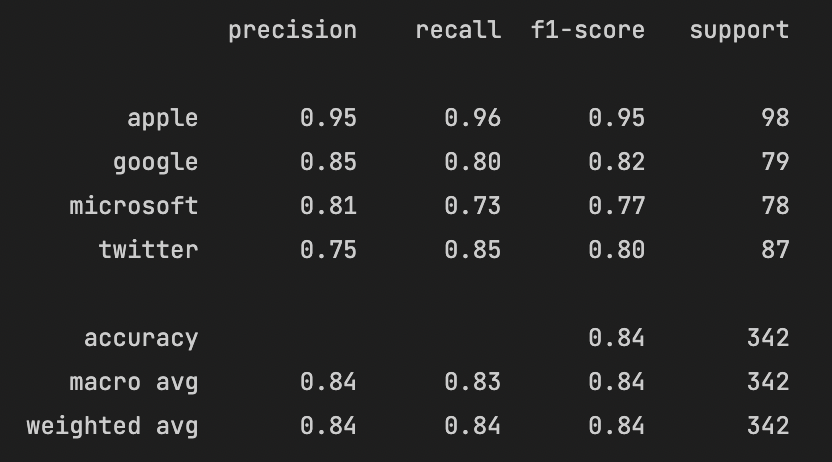
\includegraphics[height=0.56\textheight]{pic/organization.png}}
            \only<2>{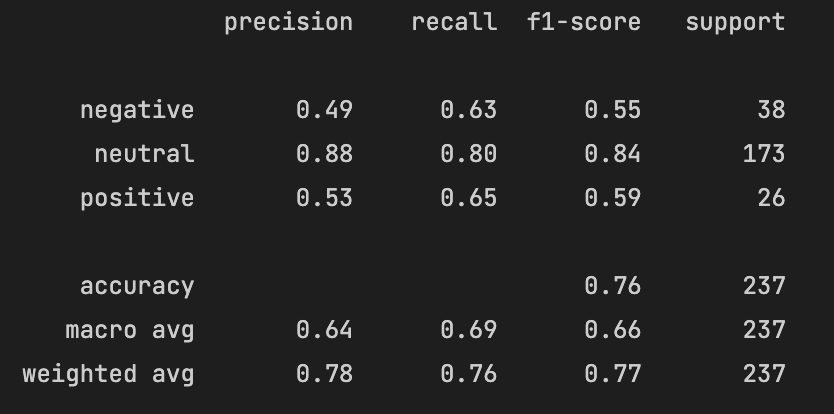
\includegraphics[height=0.5\textheight]{pic/sentiment.png}}
          \end{overprint}
        }
    \end{columns}
\end{frame}

\begin{frame}[plain]
    \itmopolygons{
        \vfill
        \Huge{Thank you for your attention!}
        \vfill
        
\includegraphics[scale=.5]{itmo/slogan.pdf}
    }
\end{frame}

\end{document}
